% Copia histórica de septiembre de 2026, anterior a la revisión de noviembre.
\documentclass[10pt,conference,a4paper]{elektron}
\usepackage[utf8]{inputenc}
\usepackage[T1]{fontenc}
\usepackage[spanish,es-tabla]{babel}
\usepackage[compress]{cite}
\usepackage{graphicx,amsmath,booktabs}
\usepackage[hidelinks]{hyperref}
\usepackage[top=3cm,headheight=2.5cm,bottom=3cm,footskip=2cm,left=1.60cm,right=1.60cm]{geometry}
\graphicspath{{figures/}{../figures/}}
\newcommand{\fpA}{\texttt{0x101000056010407}}
\newcommand{\fpB}{\texttt{0x101000016010407}}
\newcommand{\pendiente}[1]{\textbf{[Por confirmar: #1]}}
\begin{document}
\title{Implementación de detectores YOLO cuantizados en Kria KV260: partición CPU/DPU y caracterización de una plataforma propia\\[0.3cm]
\large Quantized YOLO Deployment on Kria KV260: CPU/DPU Partitioning and Characterization of a Custom Platform}
\author{
\IEEEauthorblockN{Demian N. Mozo\IEEEauthorrefmark{2}$^1$, 
Lucas A. Rabioglio\IEEEauthorrefmark{2}$^2$, 
María Celeste Cebedio\IEEEauthorrefmark{2}$^3$,
Luciana De Micco\IEEEauthorrefmark{3}\IEEEauthorrefmark{2}$^4$\vspace{0.2cm}}

\IEEEauthorblockA{\IEEEauthorrefmark{2}\emph{Instituto de Investigaciones Cient\'ificas y Tecnol\'ogicas en Electr\'onica (ICYTE)}\\\emph{Mar del Plata, Buenos Aires, Argentina}}

\IEEEauthorblockA{$^1$\texttt{\small{dmozo@alumnos.fi.mdp.edu.ar}}\\$^2$\texttt{\small{lucas.rabioglio@fi.mdp.edu.ar}}\\$^3$\texttt{\small{celestecebedio@fi.mdp.edu.ar}}}

\IEEEauthorblockA{\IEEEauthorrefmark{3}\emph{Consejo Nacional de Investigaciones Cient\'{\i}ficas y T\'ecnicas (CONICET)}\\\emph{Mar del Plata, Buenos Aires, Argentina}\\$^4$\texttt{\small{ldemicco@fi.mdp.edu.ar}}}}
\maketitle
\thispagestyle{empty}\pagestyle{empty}
\renewcommand{\abstractname}{Resumen}
\begin{abstract}
Se presenta un flujo de implementación de detectores YOLO cuantizados a INT8 en una AMD Kria KV260 y la caracterización de una plataforma propia basada en el IP DPUCZDX8G v4.1 B4096. El estudio utiliza ecogramas de un conjunto reducido cuya clase objetivo está asociada a merluza y distingue la evaluación de precisión de la evaluación del despliegue. En la plataforma histórica, YOLOv8n se particionó en 57 subgrafos DPU y 70 CPU, mientras que YOLOv7-tiny requirió un subgrafo DPU y tres conversiones en CPU. Aunque este último presenta más operaciones convolucionales, su latencia media de pipeline fue de 459,138 ms frente a 3544,368 ms. La nueva plataforma se integró mediante Vivado/Vitis 2022.2, con URAM y LeakyReLU habilitadas, y cerró timing con WNS de 0,006 ns para los clocks solicitados de 300/600 MHz. El modelo recompilado para su fingerprint produjo salidas idénticas a la simulación INT8 en nueve tensores correspondientes a tres entradas retenidas. La latencia fue de 460,139 ms por imagen en el pipeline y 42,196 ms en hardware DPU. La potencia media medida en VCC\_SOM fue de 5,721 W y la energía total aproximada medida sobre ese riel fue de 2,634 J por imagen; no corresponde a la placa completa ni a la alimentación de red. En el despliegue evaluado, el conteo de MACs convolucionales por sí solo no predijo la latencia extremo a extremo. Aunque YOLOv7-tiny requirió más MACs y presentó un tiempo de DPU ligeramente mayor, su grafo se concentró en un único subgrafo DPU y evitó el elevado costo de ejecución CPU y las numerosas transiciones observadas en YOLOv8n.
\end{abstract}
\renewcommand{\IEEEkeywordsname}{Palabras clave}
\begin{IEEEkeywords}FPGA, Kria KV260, cuantización INT8, DPU, YOLO, ecogramas.\end{IEEEkeywords}
\renewcommand{\abstractname}{Abstract}
\begin{abstract}
This work presents an INT8 YOLO deployment flow on AMD Kria KV260 and characterizes a custom platform integrating the DPUCZDX8G v4.1 B4096 IP. On the historical platform, YOLOv8n required 57 DPU and 70 CPU subgraphs, whereas YOLOv7-tiny required one DPU subgraph and three CPU conversions. Despite its larger convolutional MAC count, YOLOv7-tiny achieved a mean pipeline latency of 459.138 ms versus 3544.368 ms. The custom platform was implemented with Vivado/Vitis 2022.2, enabled URAM and LeakyReLU, and met timing with a 0.006 ns WNS at requested clocks of 300/600 MHz. After compilation for the new fingerprint, hardware outputs exactly matched retained INT8 simulation outputs across nine tensors from three echograms. Mean pipeline and DPU hardware latencies were 460.139 ms and 42.196 ms, respectively. Measured VCC\_SOM power averaged 5.721 W, with an approximate total energy of 2.634 J per image measured on that rail, excluding the full carrier board and AC mains supply. On the evaluated deployment, convolutional MAC count alone did not predict end-to-end latency. Although YOLOv7-tiny required more MACs and slightly longer DPU execution, its graph mapped to a single DPU subgraph, avoiding the substantial CPU execution cost and numerous transitions observed for YOLOv8n. These results are specific to the evaluated flow; the small dataset lacks an independent test set, and functional agreement is restricted to the retained inputs.
\end{abstract}
\renewcommand{\IEEEkeywordsname}{Keywords}
\begin{IEEEkeywords}FPGA, Kria KV260, INT8 quantization, DPU, YOLO, echograms.\end{IEEEkeywords}

\section{Introducción}
La detección automática en ecogramas plantea un problema de procesamiento embebido en el que interesa tanto el comportamiento del detector como el costo de ejecutarlo cerca de la adquisición. Una red compacta en número de parámetros u operaciones no necesariamente utiliza de manera eficiente un acelerador concreto. Cuando parte de sus operadores se ejecuta en el procesador anfitrión, el tiempo observado incluye conversiones, transferencias y coordinación entre subgrafos, además del cálculo acelerado.

El trabajo presentado en CASE abordó la detección de merluza con YOLO y su orientación hacia sistemas embebidos~\cite{mozo2026case}. Este artículo amplía ese antecedente mediante evidencia de ejecución INT8 en una KV260, diagnóstico de la partición CPU/DPU y una implementación propia de la plataforma de aceleración. La contribución de hardware comprende la integración, configuración, implementación y caracterización del IP oficial; no consiste en el diseño de una DPU nueva. Las mediciones de la plataforma construida se mantienen separadas de las obtenidas previamente con una plataforma precompilada.

El objetivo es establecer una cadena trazable desde el modelo cuantizado hasta los artefactos implementados y su ejecución, y examinar si el conteo de operaciones convolucionales resulta suficiente para explicar la latencia. Se estudian dos implementaciones históricas, YOLOv8n y YOLOv7-tiny, y se valida esta última en la nueva plataforma. La precisión se presenta como resultado secundario sobre validación interna, sin comparar métricas obtenidas con particiones de datos incompatibles.

Los aportes son: a) un flujo documentado de cuantización, compilación y despliegue asociado al fingerprint del hardware; b) un diagnóstico cuantitativo de operadores y fragmentación CPU/DPU; c) la implementación de una plataforma B4096 con reportes propios de recursos, timing y potencia estimada; y d) su validación funcional, temporal y energética con entradas retenidas y un protocolo común.

\section{Antecedentes y alcance}
YOLOv7 propone una familia de detectores y estrategias de entrenamiento~\cite{wang2023yolov7}. Aquí se utiliza la variante tiny del repositorio fijado~\cite{yolov7repo}, con activaciones LeakyReLU. El interés no está en trasladar al caso acústico los resultados de precisión o velocidad de otros conjuntos, sino en evaluar la ejecución del grafo concreto exportado. YOLOv8n se conserva como comparación histórica del comportamiento de otra arquitectura en el mismo flujo de aceleración. La versión de Ultralytics registrada en el entorno retenido es 8.4.46~\cite{ultralytics}; se cita la implementación de software y no un artículo de YOLOv8 inexistente en la evidencia. Se trata del grafo adaptado retenido, con salida cruda y transformaciones de compilación en C2f; no de una ejecución del modelo original sin cambios. El alcance de esas adaptaciones se conserva en la documentación experimental, sin atribuirles aquí una equivalencia universal.

Vitis AI separa la cuantización del modelo, la compilación orientada al acelerador y la ejecución mediante su runtime~\cite{vitisai}. Por ello, la compatibilidad debe comprobarse en el grafo compilado y en la placa; la exportación correcta de una red no demuestra que todos sus operadores se ejecuten en la DPU. En este estudio, la descomposición asociada a SiLU en YOLOv8n deja operaciones de tipo sigmoid y conversiones en CPU. En YOLOv7-tiny, el grafo resultante concentra el cálculo de la red en una DPU y conserva tres conversiones de salida en CPU.

La relación entre precisión numérica y eficiencia debe evaluarse sobre el hardware de destino. Jacob et al.~\cite{jacob2018} estudian cuantización de pesos y activaciones para inferencia con aritmética entera y un procedimiento de entrenamiento asociado. Aquí se emplea PTQ retenida, sin trasladar a este detector sus resultados de exactitud ni su estrategia de entrenamiento. LPYOLO~\cite{lpyolo} rediseña TinyYOLOv3 para detección de rostros, con Brevitas/FINN y precisiones reducidas sobre PYNQ-Z2. Ese enfoque muestra una alternativa de implementación especializada; difiere de integrar un IP DPU configurable y compilar para su conjunto de operadores.

También existen propuestas que combinan convoluciones en FPGA y posprocesamiento en software, como Hybrid YOLO FPGA~\cite{hybridyolo}. Embedded YOLO~\cite{embeddedyolo} aborda el diseño de una red ligera para vehículos pequeños, mediante cambios en backbone, cuello y cabeza; constituye un antecedente de selección arquitectónica embebida, no una validación de DPUCZDX8G. No se comparan sus cifras de velocidad, exactitud o potencia con las de este trabajo, porque difieren en datos, resolución, hardware y alcance de la medición.

En el dominio acústico, Brautaset et al.~\cite{brautaset2020} estudian clasificación con redes convolucionales sobre datos de ecosonda multifrecuencia, incluyendo estrategias para desbalance de clases, anotaciones y separación temporal de datos. Ese contexto destaca la importancia de la procedencia acústica y la validación independiente. Su tarea de clasificación por píxel y sus datos no son equivalentes a las cajas de una clase usadas aquí, por lo que tampoco se trasladan sus métricas.

La plataforma física KV260 incorpora un módulo K26~\cite{kv260}. La guía PG338 documenta el IP DPUCZDX8G y sus opciones~\cite{dpuguide}; VART proporciona las interfaces de ejecución del grafo~\cite{vart}, mientras que XRT facilita la comunicación entre la aplicación anfitriona y los aceleradores de la lógica reconfigurable~\cite{xrt}. Esta separación permite distinguir soporte del operador, compilación y costo observado durante la ejecución.

El ejemplo oficial de benchmark KV260 proporciona el punto de partida para integrar el acelerador con una plataforma existente~\cite{kria}. Se reutiliza esa estructura, incluidos sus bloques auxiliares, para evitar introducir una plataforma mínima distinta de la referencia. Los resultados de utilización describen por separado el diseño completo y la jerarquía DPU. No se pretende aislar experimentalmente el efecto de una única activación: las dos redes también difieren en topología, cabezas y posprocesamiento.

\section{Datos, modelo y cuantización}
\subsection{Conjunto acústico y partición}
Se trabajó con ecogramas anotados para una clase objetivo asociada a merluza en el conjunto anotado. El archivo de configuración la denomina \texttt{fish}; el antecedente CASE, sección II-A, establece que esa etiqueta identifica ecos asociados a merluza en las imágenes disponibles~\cite{mozo2026case}. Se conserva esa asociación documental, sin convertirla en una identificación biológica independiente ni en una validación de discriminación entre especies. Las imágenes son representaciones acústicas y su apariencia depende del procesamiento de adquisición; no se atribuyen unidades físicas a sus intensidades RGB. La evidencia disponible no permite completar de manera inequívoca la procedencia de toda la campaña, la calibración acústica ni la independencia entre maniobras. Por tanto, la evaluación describe este conjunto retenido y no establece generalización a otras campañas.

La auditoría del árbol experimental de YOLOv7-tiny identifica 84 archivos: 59 para entrenamiento (P1--P60, excepto P39), cinco excluidos como separación secuencial (P61--P65), 18 de validación (P66--P83) y dos archivos asociados al identificador conflictivo P39, también excluidos. Sus anotaciones son, respectivamente, 1688, 103, 548 y 75 cajas. La separación secuencial reduce la proximidad inmediata entre entrenamiento y validación, pero no prueba independencia de campaña. No existe un conjunto de prueba independiente. El recuento de 85 imágenes del antecedente CASE no se utiliza como denominador de esta evaluación: corresponde a documentación previa cuya diferencia de inventario permanece pendiente de conciliación.

\subsection{Entrenamiento retenido y PTQ}
El modelo YOLOv7-tiny contiene 6\,014\,038 parámetros. Se conserva la arquitectura \texttt{cfg/deploy/yolov7-tiny.yaml} del commit \texttt{eef4f2c} del repositorio original. El entrenamiento retenido utilizó semilla 42, SGD, batch de cuatro y 121 épocas, con 1815 actualizaciones del optimizador, en FP32 y con AMP y TF32 desactivados. El checkpoint seleccionado por mAP@0,5:0,95 de validación corresponde a la media móvil exponencial de la época 81, con 1215 actualizaciones. Esta selección es una razón adicional para interpretar las métricas como validación interna.

La cuantización posterior al entrenamiento (PTQ) produjo el modelo INT8 previo a compilación \texttt{TinyRaw\_int.xmodel}. La calibración utilizó las 59 imágenes de entrenamiento; la validación no formó parte de ella. Se retienen las salidas de simulación y la evaluación FP32/INT8 existentes; la construcción de la plataforma propia no incluyó reentrenamiento, recalibración, QAT ni modificación de la red. LeakyReLU utiliza pendiente nominal 0,1, con representación cuantizada 0,1015625 en el flujo retenido.

Se informa precisión, exhaustividad, mAP@0,5 y mAP@0,5:0,95 sobre las mismas 18 imágenes. Precisión y exhaustividad se calculan en el punto de confianza 0,25, con NMS IoU de 0,6; la mAP resume la curva correspondiente y no debe interpretarse como una métrica definida exclusivamente en ese punto. El umbral alternativo 0,2147436, derivado de validación en un análisis anterior, no se utiliza en el benchmark final.

\section{Flujo de implementación y plataforma propia}
\subsection{Separación entre software y hardware}
La Fig.~\ref{fig:pipeline} distingue las funciones del sistema de procesamiento ARM (PS) y de la lógica programable (PL). En ARM se realiza el preprocesamiento, se cuantiza y copia el tensor de entrada, y se invoca Graph Runner. La DPU ejecuta el subgrafo acelerado; tres operaciones \texttt{fix2float} convierten las cabezas de salida antes de la decodificación, NMS y transformación de coordenadas en ARM.

\begin{figure*}[t]
\centering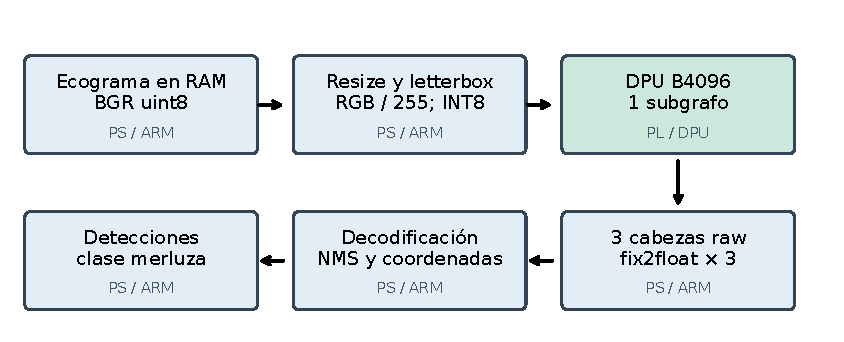
\includegraphics[width=.9\textwidth]{pipeline.pdf}
\caption{Pipeline de YOLOv7-tiny. La medición comienza con la imagen decodificada en RAM. Graph Runner comprende la DPU, las conversiones CPU y la coordinación de ejecución; no incluye todo el preprocesamiento ni el posprocesamiento.}\label{fig:pipeline}
\end{figure*}

La cadena de artefactos tiene dos ramas convergentes. La rama de software parte de PyTorch, pasa por PTQ INT8 y genera un XMODEL previo a compilación. La rama de hardware integra el IP DPU con la plataforma base mediante Vivado/Vitis y produce bitstream, XSA, XCLBIN y \texttt{arch.json}. Este último fija el destino de \texttt{vai\_c\_xir}, que compila el XMODEL para esa configuración. El despliegue reúne BIN, DTBO, XCLBIN y \texttt{shell.json} bajo una aplicación diferenciada y ejecuta el modelo mediante VART. Los hashes permiten vincular cada resultado con los artefactos empleados.

Se distinguen la plataforma histórica A, fingerprint \fpA, y la propia B, fingerprint \fpB. Aunque ambas se identifican como B4096, los fingerprints difieren; por ello no se reutilizó silenciosamente el compilado anterior ni se atribuyeron a A los recursos de B. La diferencia se asocia a la configuración de \texttt{SAVE\_ARGMAX\_ENA} en la auditoría de los parámetros, sin suponer equivalencia general entre plataformas.

\subsection{Configuración e implementación}
La plataforma B se construyó con Vivado 2022.2, build 3671981, y Vitis 2022.2, build 3671529, a partir de la rama \texttt{xlnx\_rel\_v2022.2} de \texttt{kria-vitis-platforms}, commit \texttt{a3a83f1}. Se utilizó el IP oficial distribuido para Vitis AI 3.0: \texttt{xilinx.com:ip:dpuczdx8g:4.1}, revisión 0. Su envoltorio de kernel Vitis tiene VLNV \nolinkurl{xilinx.com:RTLKernel:DPUCZDX8G:1.0}; ambas numeraciones identifican componentes distintos.

La configuración comprende una DPU B4096, URAM habilitada y LeakyReLU habilitada en convolución. El parámetro de LeakyReLU de ALU permanece deshabilitado. Se solicitaron 300 MHz para \texttt{aclk} y 600 MHz para \texttt{ap\_clk\_2}. Los metadatos del XCLBIN registran 299,997 y 599,994 MHz; la consulta conservada dentro de la traza de ejecución informa 300 MHz para DPU y XRT. Son frecuencias nominales o reportadas por herramientas, no una medición de frecuencia máxima alcanzable.

Se completó una construcción oficial, sin detener artificialmente el enlace, conservando proyecto, checkpoint ruteado, logs y artefactos. La Tabla~\ref{tab:resources} muestra la utilización post-route. LUTRAM y SRL son subcategorías incluidas en LUT; no se suman nuevamente al total. El diseño completo conserva los bloques de la plataforma base, por lo que su costo no equivale al costo aislado del detector. El reporte \texttt{report\_utilization} del dispositivo \nolinkurl{xck26-sfvc784-2LV-c} informa para ese diseño 59,43\% de LUT, 55,40\% de registros utilizados como FF, 65,63\% de bloques BRAM, 87,50\% de URAM y 56,89\% de DSP. Se retienen los valores absolutos de ambas jerarquías en la tabla para preservar su legibilidad; los porcentajes citados corresponden al diseño completo y no a la DPU aislada.

\begin{table}[t]
\caption{Recursos post-route de la plataforma B.}\label{tab:resources}
\centering\small\begin{tabular}{lrr}\toprule
Recurso & Diseño completo & Jerarquía DPU\\\midrule
LUT & 69610 & 51291 \\
FF & 129766 & 96711 \\
LUTRAM & 3056 & 2736 \\
SRL & 5098 & 4297 \\
RAMB36 & 88 & 70 \\
RAMB18 & 13 & 10 \\
BRAM (equiv. 36 Kib) & 94,5 & 75 \\
URAM & 56 & 48 \\
DSP & 710 & 710 \\
\bottomrule\end{tabular}
\end{table}

El análisis temporal presenta WNS de $+0{,}006$ ns y TNS de cero; WHS de $+0{,}010$ ns y THS de cero; y WPWS de $+0{,}071$ ns. Las 12 restricciones de bus skew tienen un margen mínimo de $+1{,}979$ ns. Se registran 207\,743 redes completamente ruteadas y ningún error de ruteo. La comprobación independiente de DRC informa cero errores y cero advertencias críticas, junto con 580 advertencias ordinarias. Persisten avisos de metodología sobre retardos de entrada I\textsuperscript{2}C ausentes, caminos multiciclo y señales CE, resets asíncronos de MIPI y utilización de DSP. El cierre temporal se limita a las restricciones aplicadas y su margen de setup es reducido.

La estimación postimplementación de potencia de Vivado es de 7,026 W sobre el chip: 6,666 W dinámicos y 0,360 W estáticos. Es una estimación sin actividad de simulación (\emph{vectorless}), de confianza baja. Se presenta separadamente de la medición de VCC\_SOM; difieren tanto el método como el alcance eléctrico.

\subsection{Compilación y despliegue trazables}
El modelo INT8 se compiló con Vitis AI 3.0 y el \texttt{arch.json} de B. El compilador informó el destino \nolinkurl{DPUCZDX8G_ISA1_B4096_0101000016010407}. La auditoría conservada identifica un subgrafo USER de entrada, uno DPU y tres CPU. Las operaciones DPU comprenden 58 \texttt{conv2d-fix}, 14 \texttt{concat-fix}, seis \texttt{pool-fix}, dos \texttt{upsample-fix}, 116 constantes, una carga y tres descargas. Los tres subgrafos CPU contienen una conversión \texttt{fix2float} cada uno. La comparación con el compilado histórico conserva esta estructura, entradas, salidas y posiciones de punto fijo; cambia el fingerprint de destino.

La entrada es INT8 en orden NHWC, de forma $1\times1024\times1024\times3$ y posición de punto fijo 6. Las salidas DPU tienen 18 canales y resoluciones $128^2$, $64^2$ y $32^2$, con posiciones de punto fijo 1, 2 y 1. Graph Runner entrega sus versiones float32. Esta interfaz permite conservar el ejecutor existente.

La aplicación \texttt{kv260-elektron-b4096-v41} se empaquetó separadamente de la histórica. Para el DTBO se retuvo el overlay funcional y se modificó únicamente el nombre del firmware; la descompilación de comprobación conserva, entre otras propiedades, \texttt{fpga-config-from-dmabuf}. La traza VART de la campaña B confirma el fingerprint nuevo, una DPU v4.1 y la frecuencia nominal de 300 MHz. El UUID del XCLBIN queda registrado en los metadatos del paquete. La compilación y los artefactos de A se conservan como referencia independiente.

\section{Protocolo experimental}
\subsection{Latencia y particionamiento}
Se procesaron P66, P74 y P83 a resolución $1024\times1024$, batch uno, diez calentamientos y cien ejecuciones medidas, alternando las tres imágenes. Las imágenes BGR uint8 estaban decodificadas y precargadas en RAM; lectura de archivo, decodificación PNG y adquisición acústica quedan fuera del intervalo. Se mantuvo el preprocesamiento cuadrado con reducción AREA, dimensiones enteras, relleno gris 114, conversión a RGB float32 NCHW y división por 255. La entrada de la DPU se obtuvo mediante escalado por $2^6$, redondeo, saturación INT8 y copia a NHWC.

El pipeline fue secuencial, sin solapamiento ni optimización adicional de copias. Se fijó un hilo de OpenCV y de BLAS; el protocolo registra CPU en modo userspace a 1\,333\,333 kHz. La ejecución utiliza AMD Kria KV260 con módulo K26. El inventario previo al cambio de plataforma registra PetaLinux 2022.2 (\nolinkurl{2022.2_release_S10071807}, honister), kernel Linux \nolinkurl{5.15.36-xilinx-v2022.2}, arquitectura aarch64 y XRT/ZOCL 2.14.0, commit \texttt{43926231}. El protocolo B conserva ese entorno sin actualización del sistema; no se dispone de una segunda captura completa del sistema operativo posterior al cambio. La traza B sí confirma VART 3.0.0, XIR commit \texttt{9204ac72} y DPU a 300 MHz nominales, y los JSON del benchmark registran OpenCV 4.5.2 y NumPy 1.21.2. La traza informa el ARM a 1333 MHz, consistente con los 1\,333\,333 kHz del protocolo. Se realizaron una pasada normal y otra perfilada de cien imágenes, ambas posteriores al calentamiento. La normal proporciona tiempos del pipeline y telemetría de potencia; la perfilada permite separar hardware DPU, controlador DPU y subgrafos CPU. No se suman tiempos de pasadas distintas.

Se informa media, mediana, desviación estándar muestral y percentil 95. La latencia hardware DPU se obtiene del contador de la traza y la frecuencia nominal. Los porcentajes respecto de Graph Runner o del pipeline utilizan siempre el denominador de la misma pasada perfilada. Los conteos de subgrafos y operadores provienen del grafo; las transiciones ejecutadas, de la secuencia temporal. Los bytes de frontera corresponden a tamaños lógicos de tensores, no a tráfico físico de DRAM medido.

\subsection{Paridad funcional}
Para evitar diferencias de resize entre implementaciones de OpenCV, se compararon las salidas de B con la simulación INT8 retenida que utilizó exactamente los mismos tensores preprocesados en ARM. Se conservaron entradas y hashes. Para cada una de las tres imágenes se evaluaron tres cabezas raw, expresadas en NCHW. Se calcularon error absoluto máximo, RMSE y cantidad de elementos distintos. Esta comprobación de nueve tensores es independiente de la evaluación de precisión sobre las 18 imágenes; no amplía el conjunto de validación ni demuestra paridad para entradas arbitrarias.

\subsection{Potencia y energía}
La medición utiliza el sensor INA260 U14, asociado a VCC\_SOM. Su alcance es el módulo SOM y no la placa portadora completa ni la potencia tomada de la red eléctrica. La pasada normal conserva 30 lecturas de reposo anteriores, 92 durante inferencia y 30 posteriores, con intervalo objetivo de 0,5 s y aproximadamente 15 s en cada tramo de reposo.

Se integra la potencia mediante trapecios sobre el intervalo medido, extendiendo la primera y la última lectura activa hasta sus extremos. Para $N=100$ imágenes y duración $T$, se define
\begin{equation}
E_{\mathrm{img}}=\frac{1}{N}\int_0^T P(t)\,dt,\qquad
\bar P=\frac{N E_{\mathrm{img}}}{T}.
\end{equation}
La energía incremental resta $P_0T/N$, donde $P_0$ es la media aritmética de las lecturas de reposo anteriores y posteriores. Se trata de una aproximación telemétrica de la ejecución completa, no de una medición aislada de energía de la DPU.

\section{Resultados}
\subsection{Precisión interna retenida}
La Tabla~\ref{tab:accuracy} presenta la evaluación de YOLOv7-tiny sobre 18 imágenes y 548 cajas. La cuantización conserva valores próximos de precisión y exhaustividad; mAP@0,5 aumenta 0,003 y mAP@0,5:0,95 disminuye 0,016 en escala unitaria. Estos cambios describen esta validación y no prueban una mejora de generalización. Los resultados históricos de precisión de YOLOv8n se obtuvieron con otro conjunto y no se incorporan a una comparación directa de exactitud.

\begin{table}[t]\caption{YOLOv7-tiny: validación interna común. P y R a confianza 0,25; NMS IoU 0,6.}\label{tab:accuracy}
\centering\small\begin{tabular}{lrr}\toprule
Métrica & FP32 & Simulación INT8\\\midrule
Precisión (P) & 0,714 & 0,722\\
Exhaustividad (R) & 0,624 & 0,630\\
mAP@0,5 & 0,674 & 0,677\\
mAP@0,5:0,95 & 0,277 & 0,262\\
Falsos positivos & 137 & 133\\
Falsos negativos & 206 & 203\\\bottomrule\end{tabular}
\end{table}

\subsection{Fragmentación y rendimiento histórico}
En A, YOLOv8n contiene 57 subgrafos DPU y 70 CPU, con 113 transiciones ejecutadas por imagen. Los subgrafos CPU incluyen 70 \texttt{fix2float}, 64 \texttt{float2fix} y 64 \texttt{sigmoid}. Las fronteras CPU/DPU representan 70\,865\,920 bytes lógicos. YOLOv7-tiny presenta un subgrafo DPU, tres CPU y una transición de dispositivo en la secuencia ejecutada, con 387\,072 bytes lógicos de frontera. La Fig.~\ref{fig:partition} muestra los conteos en una escala común; no los interpreta como porcentajes de operaciones ni de tiempo.

\begin{figure}[t]\centering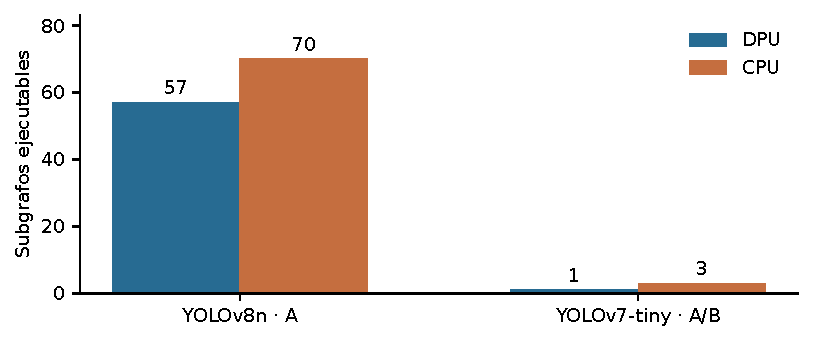
\includegraphics[width=\columnwidth]{partition.pdf}
\caption{Partición de los grafos. YOLOv8n fue medido en A; YOLOv7-tiny conserva el conteo en A y B. USER no se cuenta como subgrafo ejecutable.}\label{fig:partition}\end{figure}

El conteo convolucional es 10,345 GMAC para YOLOv8n y 16,667 GMAC para YOLOv7-tiny. Sin embargo, el pipeline normal de YOLOv8n tarda 3544,368 ms y el de YOLOv7-tiny 459,138 ms: una razón de 7,72 en favor de este último para esas implementaciones. En la pasada perfilada, YOLOv8n dedica 36,623 ms al hardware DPU y 2935,837 ms a subgrafos CPU; estos últimos representan el 96,92\% de Graph Runner. En YOLOv7-tiny, esos tiempos son 42,182 y 0,585 ms, respectivamente. La ventaja del pipeline no proviene de un menor tiempo de cálculo DPU.

\begin{figure*}[t]\centering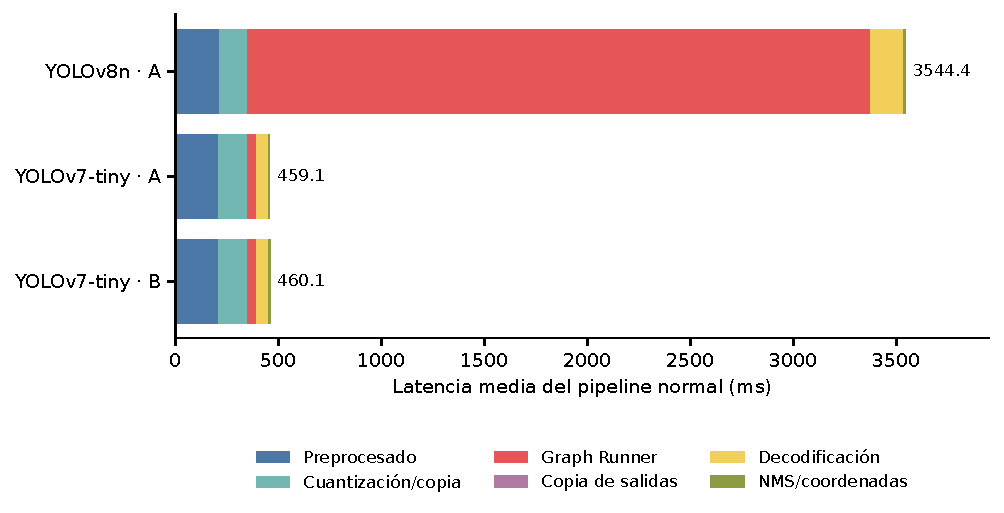
\includegraphics[width=.9\textwidth]{latency.pdf}
\caption{Descomposición de la latencia normal con eje lineal común. Las dos primeras filas comparan modelos en A; la tercera valida YOLOv7-tiny en B. Graph Runner incluye coordinación y conversiones, además de ejecución DPU.}\label{fig:latency}\end{figure*}

\subsection{Validación de la plataforma propia}
La comparación offline de los archivos retenidos confirma igualdad numérica exacta en los nueve tensores raw (Tabla~\ref{tab:parity}). Error máximo, RMSE y cantidad de valores distintos son cero en cada caso. En la pasada normal del benchmark, a confianza 0,25, se registran 17, 27 y 25 detecciones para P66, P74 y P83, respectivamente; la pasada perfilada conserva esos conteos. No se confunden con los conteos obtenidos anteriormente usando otro umbral de confianza.

\begin{table}[t]\caption{Paridad B frente a simulación INT8 con entradas ARM idénticas. Cero elementos distintos en todos los casos.}\label{tab:parity}
\centering\small\begin{tabular}{lcrr}\toprule
Entrada & Forma NCHW & Error máx. & RMSE\\\midrule
P66 & $1\!\times\!18\!\times\!128\!\times\!128$ & 0 & 0 \\
P66 & $1\!\times\!18\!\times\!64\!\times\!64$ & 0 & 0 \\
P66 & $1\!\times\!18\!\times\!32\!\times\!32$ & 0 & 0 \\
P74 & $1\!\times\!18\!\times\!128\!\times\!128$ & 0 & 0 \\
P74 & $1\!\times\!18\!\times\!64\!\times\!64$ & 0 & 0 \\
P74 & $1\!\times\!18\!\times\!32\!\times\!32$ & 0 & 0 \\
P83 & $1\!\times\!18\!\times\!128\!\times\!128$ & 0 & 0 \\
P83 & $1\!\times\!18\!\times\!64\!\times\!64$ & 0 & 0 \\
P83 & $1\!\times\!18\!\times\!32\!\times\!32$ & 0 & 0 \\
\bottomrule\end{tabular}\end{table}

La traza contiene 440 intervalos de ejecución emparejados, correspondientes a $(10+100)\times(1+3)$ subgrafos. Tras excluir los calentamientos, el tiempo medio de hardware DPU es 42,196 ms y el del controlador 42,328 ms. Las conversiones CPU suman 0,583 ms. La Tabla~\ref{tab:latency} presenta las distribuciones; los tiempos del controlador contienen la ejecución hardware y no deben sumarse a ella.

\begin{table*}[t]\caption{Latencias de B en ms, cien ejecuciones. Las primeras siete filas corresponden a la pasada normal; las últimas tres, al perfilado independiente. DE: desviación estándar muestral.}\label{tab:latency}
\centering\small\begin{tabular}{lrrrr}\toprule
Etapa & Media & Mediana & DE & p95\\\midrule
Preprocesado & 212,282 & 212,213 & 0,730 & 213,544 \\
Cuantización/copia & 137,119 & 136,824 & 1,051 & 139,237 \\
Graph Runner & 45,903 & 45,895 & 0,065 & 45,963 \\
Copia de salidas & 0,980 & 0,973 & 0,030 & 1,039 \\
Decodificación & 57,056 & 57,029 & 0,219 & 57,389 \\
NMS/coordenadas & 6,800 & 7,029 & 0,880 & 7,769 \\
Pipeline normal & 460,139 & 460,084 & 1,481 & 462,173 \\
DPU hardware (perfil) & 42,196 & 42,195 & 0,008 & 42,208 \\
Controlador DPU (perfil) & 42,328 & 42,329 & 0,015 & 42,350 \\
CPU (perfil) & 0,583 & 0,579 & 0,013 & 0,603 \\
\bottomrule\end{tabular}\end{table*}

El pipeline normal alcanza 460,139 ms y Graph Runner 45,903 ms. En el perfilado, el pipeline registra 459,165 ms y Graph Runner 46,027 ms. La diferencia entre pasadas es $-0,212$\%; no representa una aceleración causada por instrumentar. El tiempo DPU constituye el 91,68\% de Graph Runner y el 9,19\% del pipeline perfilado. No se observa solapamiento positivo entre los intervalos ejecutados.

\subsection{Potencia y comparación A/B}
En B, los reposos anterior y posterior promedian 5,002 y 4,990 W, respectivamente. La media temporal durante inferencia es 5,721 W; la desviación estándar de las 92 lecturas activas es 1,119 W. El intervalo de cien imágenes dura 46,039 s y produce 2,634 J por imagen, o 0,334 J por imagen tras restar el reposo medio. La duración incluye el pequeño costo de control entre iteraciones, además de las etapas cronometradas individualmente.

\begin{table*}[t]\caption{YOLOv7-tiny en A y B. Diferencia relativa: $100(B/A-1)$. Se comparan métricas de igual alcance; los tiempos de subgrafos proceden del perfilado. Fingerprints: A = \fpA; B = \fpB.}\label{tab:ab}
\centering\small\begin{tabular}{lrrr}\toprule
Métrica & A histórica & B propia & Diferencia (\%)\\\midrule
Pipeline normal (ms) & 459,138 & 460,139 & 0,22 \\
Graph Runner normal (ms) & 45,925 & 45,903 & -0,05 \\
DPU hardware perfilada (ms) & 42,182 & 42,196 & 0,03 \\
Controlador DPU (ms) & 42,317 & 42,328 & 0,03 \\
Subgrafos CPU (ms) & 0,585 & 0,583 & -0,35 \\
Reposo SOM (W) & 5,026 & 4,996 & -0,60 \\
Inferencia SOM (W) & 5,741 & 5,721 & -0,36 \\
Energía total (J/imagen) & 2,638 & 2,634 & -0,14 \\
Energía incremental (J/imagen) & 0,328 & 0,334 & 1,60 \\
\bottomrule\end{tabular}\end{table*}

La Tabla~\ref{tab:ab} muestra diferencias de aproximadamente $+0,22$\% en pipeline normal, $+0,03$\% en hardware DPU y $-0,14$\% en energía total. Son observaciones de cercanía entre las pasadas retenidas, no una demostración de equivalencia estadística ni de superioridad de B. La energía incremental resulta más sensible a la referencia de reposo. Como contexto histórico, YOLOv8n en A registró 5,398 W durante inferencia y 19,143 J por imagen: una potencia algo menor puede coexistir con mayor energía cuando la ejecución es mucho más larga.

\section{Discusión y limitaciones}
En el despliegue evaluado, el conteo de MACs convolucionales por sí solo no predijo la latencia extremo a extremo. Aunque YOLOv7-tiny requirió más MACs y presentó un tiempo de DPU ligeramente mayor, su grafo se concentró en un único subgrafo DPU y evitó el elevado costo de ejecución CPU y las numerosas transiciones observadas en YOLOv8n. La evidencia del perfilado permite localizar ese costo en subgrafos CPU asociados a la descomposición del grafo. No permite asignar causalmente toda la diferencia a SiLU, al número de transiciones o a tráfico DRAM, porque no se realizó una ablación controlada ni se midió el tráfico físico.

La plataforma propia aporta una cadena adicional de evidencia: configuración del IP, implementación ruteada, recursos, artefactos identificados por hash, compilado para su fingerprint y ejecución en placa. La paridad raw de las entradas retenidas vincula el modelo cuantizado con la ejecución nueva. Los tiempos próximos a A apoyan la consistencia práctica de esa reconstrucción para el caso evaluado. No se diseñó el procesador DPU ni se demuestra identidad general entre las dos configuraciones de hardware.

Una vez reducida la fragmentación, el cuello de botella se desplaza al software ARM. En B, preprocesamiento y cuantización/copia suman 349,401 ms en la pasada normal, antes de invocar Graph Runner. Esto señala posibles líneas futuras en el movimiento de datos y el procesamiento de entrada y salida. El presente trabajo conserva el protocolo sin esas optimizaciones para mantener comparabilidad; no extrapola una mejora que no se midió.

La precisión se limita a un conjunto pequeño, sin test independiente y con selección del checkpoint sobre la validación informada. La procedencia acústica incompleta, el conflicto P39 y la diferencia de inventario con CASE deben acompañar cualquier interpretación del detector. Las métricas de YOLOv8n no comparten el split de YOLOv7-tiny. La paridad hardware/simulación se restringe a tres entradas y nueve tensores; no sustituye una evaluación de exactitud de toda la validación ejecutada en B.

En rendimiento se utilizaron tres imágenes repetidas, una pasada normal y una perfilada por configuración. Las cien iteraciones caracterizan esa ejecución, pero no son cien sesiones independientes ni cien ecogramas distintos. No se cuantificó variabilidad entre días o condiciones ambientales, ni throughput concurrente. Las imágenes estaban en RAM; el pipeline excluye adquisición acústica, lectura y decodificación de archivos. Sin una cadencia requerida de la ecosonda, no corresponde afirmar operación en tiempo real.

La energía proviene de telemetría aproximada de VCC\_SOM y no del sistema completo. El muestreo no resuelve cada etapa individual y la resta de reposo no aísla físicamente a la DPU. La estimación vectorless de Vivado se conserva como resultado de implementación separado. Finalmente, el timing cierra con margen de setup de 6 ps y advertencias de metodología: el resultado no demuestra cierre para caminos sin restricciones adecuadas ni determina una frecuencia máxima experimental.

\section{Conclusiones}
Se consolidó y validó un flujo de despliegue INT8 desde el modelo cuantizado hasta una plataforma KV260 propia que integra DPUCZDX8G v4.1 B4096. La implementación produjo artefactos y reportes trazables, cumplió las restricciones temporales aplicadas y ejecutó un modelo compilado específicamente para su fingerprint. En tres ecogramas con entradas ARM idénticas, sus nueve tensores raw coincidieron exactamente con la simulación retenida.

El contraste histórico mostró que una red con más operaciones convolucionales puede ofrecer menor latencia de pipeline cuando su grafo se adapta mejor al acelerador. Para YOLOv7-tiny en la nueva plataforma se midieron 460,139 ms por imagen, 42,196 ms de hardware DPU y aproximadamente 2,634 J por imagen en VCC\_SOM. Estos resultados caracterizan el caso estudiado, con precisión secundaria sobre validación interna, y orientan el trabajo futuro hacia software ARM, trazabilidad acústica y evaluación con campañas independientes.

\section*{Disponibilidad de datos y materiales}
El paquete local de reproducibilidad reúne manifiestos SHA-256, muestras de latencia y potencia, trazas, reportes post-route y scripts de análisis offline. La ubicación pública y las condiciones de distribución de imágenes, pesos y artefactos de hardware quedan \pendiente{repositorio y permisos de publicación}. No se declara una disponibilidad pública aún inexistente.

\section*{Contribuciones de autoría y declaraciones}
\pendiente{roles CRediT, ORCID, financiación, agradecimientos y declaración de conflictos de interés}. Estos datos deben ser completados por los autores antes del envío.

\begin{thebibliography}{99}
\bibitem{mozo2026case}D. N. Mozo, L. Rabioglio, C. Cebedio y L. De Micco, ``Detección de Merluza en Sonar con YOLO para Sistemas Embebidos,'' trabajo presentado en el Congreso Argentino de Sistemas Embebidos (CASE), San Rafael, Mendoza, Argentina, 6--7 de agosto de 2026. Copia del manuscrito conservada; publicación en actas, DOI e ISBN específicos no confirmados.
\bibitem{wang2023yolov7}C.-Y. Wang, A. Bochkovskiy y H.-Y. M. Liao, ``YOLOv7: Trainable Bag-of-Freebies Sets New State-of-the-Art for Real-Time Object Detectors,'' en \emph{Proc. IEEE/CVF Conference on Computer Vision and Pattern Recognition}, 2023, pp. 7464--7475. doi: \href{https://doi.org/10.1109/CVPR52729.2023.00721}{10.1109/CVPR52729.2023.00721}.
\bibitem{yolov7repo}C.-Y. Wang y colaboradores, \emph{YOLOv7: implementación oficial}, repositorio WongKinYiu/yolov7, commit \texttt{eef4f2c92851}. \url{https://github.com/WongKinYiu/yolov7}.
\bibitem{ultralytics}Ultralytics, \emph{Ultralytics YOLO}, software, versión 8.4.46. \url{https://github.com/ultralytics/ultralytics/tree/v8.4.46}.
\bibitem{vitisai}AMD, \emph{Vitis AI User Guide}, UG1414, versión 3.0, 24 de febrero de 2023. \url{https://docs.amd.com/r/3.0-English/ug1414-vitis-ai/Deep-Learning-Processor-Unit}.
\bibitem{jacob2018}B. Jacob, S. Kligys, B. Chen, M. Zhu, M. Tang, A. Howard, H. Adam y D. Kalenichenko, ``Quantization and Training of Neural Networks for Efficient Integer-Arithmetic-Only Inference,'' en \emph{Proc. IEEE Conference on Computer Vision and Pattern Recognition}, 2018, pp. 2704--2713. \href{https://openaccess.thecvf.com/content_cvpr_2018/html/Jacob_Quantization_and_Training_CVPR_2018_paper.html}{Repositorio oficial CVF}.
\bibitem{lpyolo}B. G\"unay, S. B. Okcu y H. \c{S}akir Bilge, ``LPYOLO: Low Precision YOLO for Face Detection on FPGA,'' arXiv:2207.10482, 2022. \url{https://doi.org/10.48550/arXiv.2207.10482}.
\bibitem{hybridyolo}P. Saranya, P. Sowmiyaa, M. Pooja, C. Srinithi y B. Sowbarnika, ``A Hybrid Yolo FPGA Architecture for Real-Time Object Detection in Edge Computing,'' \emph{International Research Journal on Advanced Engineering Hub}, vol. 3, n.\textsuperscript{o} 3, pp. 303--306, 2025. \url{https://doi.org/10.47392/IRJAEH.2025.0042}.
\bibitem{embeddedyolo}W. Feng, J. Liu, Y. Zhu, J. Zheng y H. Wang, ``Embedded YOLO: A Real-Time Object Detector for Small Intelligent Trajectory Cars,'' \emph{Mathematical Problems in Engineering}, vol. 2021, art. 6555513, 2021. \url{https://doi.org/10.1155/2021/6555513}. Autoría según el corrigendum, art. 9818014: \url{https://doi.org/10.1155/2021/9818014}.
\bibitem{brautaset2020}O. Brautaset, A. U. Waldeland, E. Johnsen, K. Malde, L. Eikvil, A.-B. Salberg y N. O. Handegard, ``Acoustic classification in multifrequency echosounder data using deep convolutional neural networks,'' \emph{ICES Journal of Marine Science}, vol. 77, pp. 1391--1400, 2020. \url{https://doi.org/10.1093/icesjms/fsz235}.
\bibitem{kv260}AMD, \emph{Kria KV260 Vision AI Starter Kit Data Sheet}, DS986. \url{https://docs.amd.com/r/en-US/ds986-kv260-starter-kit/Ordering-Information}.
\bibitem{dpuguide}AMD, \emph{DPUCZDX8G for Zynq UltraScale+ MPSoCs Product Guide}, PG338, versión 4.1, 23 de enero de 2023. \url{https://docs.amd.com/r/en-US/pg338-dpu/Features}.
\bibitem{vart}AMD, ``Programming with VART,'' en \emph{Vitis AI User Guide}, UG1414, versión 3.0, 2023. \url{https://docs.amd.com/r/3.0-English/ug1414-vitis-ai/Programming-with-VART}.
\bibitem{xrt}AMD, \emph{Xilinx Runtime (XRT) Release Notes}, UG1451, versión 2022.2, 21 de octubre de 2022. \url{https://docs.amd.com/r/2022.2-English/ug1451-xrt-release-notes/About-Xilinx-Runtime-XRT}.
\bibitem{kria}Xilinx, \emph{Kria Vitis Platforms}, rama \texttt{xlnx\_rel\_v2022.2}, commit \texttt{a3a83f1}, ejemplo KV260 benchmark. \url{https://github.com/Xilinx/kria-vitis-platforms/tree/a3a83f179503792226adf83082aee7c05de620b4/kv260/overlays/examples/benchmark}.
\end{thebibliography}
\end{document}
